\documentclass[12pt]{article}

%packages
%\usepackage{latexsym}
\usepackage{graphicx}
\usepackage{color}
\usepackage{amsmath}
\usepackage{dsfont}
\usepackage{placeins}
\usepackage{amssymb}
\usepackage{wasysym}
\usepackage{abstract}
\usepackage{hyperref}
\usepackage{etoolbox}
\usepackage{datetime}
\usepackage{xcolor}
\usepackage{alphalph}
\settimeformat{ampmtime}

%\usepackage{pstricks,pst-node,pst-tree}

%\usepackage{algpseudocode}
%\usepackage{amsthm}
%\usepackage{hyperref}
%\usepackage{mathrsfs}
%\usepackage{amsfonts}
%\usepackage{bbding}
%\usepackage{listings}
%\usepackage{appendix}
\usepackage[margin=1in]{geometry}
%\geometry{papersize={8.5in,11in},total={6.5in,9in}}
%\usepackage{cancel}
%\usepackage{algorithmic, algorithm}

\makeatletter
\def\maxwidth{ %
  \ifdim\Gin@nat@width>\linewidth
    \linewidth
  \else
    \Gin@nat@width
  \fi
}
\makeatother

\definecolor{fgcolor}{rgb}{0.345, 0.345, 0.345}
\newcommand{\hlnum}[1]{\textcolor[rgb]{0.686,0.059,0.569}{#1}}%
\newcommand{\hlstr}[1]{\textcolor[rgb]{0.192,0.494,0.8}{#1}}%
\newcommand{\hlcom}[1]{\textcolor[rgb]{0.678,0.584,0.686}{\textit{#1}}}%
\newcommand{\hlopt}[1]{\textcolor[rgb]{0,0,0}{#1}}%
\newcommand{\hlstd}[1]{\textcolor[rgb]{0.345,0.345,0.345}{#1}}%
\newcommand{\hlkwa}[1]{\textcolor[rgb]{0.161,0.373,0.58}{\textbf{#1}}}%
\newcommand{\hlkwb}[1]{\textcolor[rgb]{0.69,0.353,0.396}{#1}}%
\newcommand{\hlkwc}[1]{\textcolor[rgb]{0.333,0.667,0.333}{#1}}%
\newcommand{\hlkwd}[1]{\textcolor[rgb]{0.737,0.353,0.396}{\textbf{#1}}}%

\usepackage{framed}
\makeatletter
\newenvironment{kframe}{%
 \def\at@end@of@kframe{}%
 \ifinner\ifhmode%
  \def\at@end@of@kframe{\end{minipage}}%
  \begin{minipage}{\columnwidth}%
 \fi\fi%
 \def\FrameCommand##1{\hskip\@totalleftmargin \hskip-\fboxsep
 \colorbox{shadecolor}{##1}\hskip-\fboxsep
     % There is no \\@totalrightmargin, so:
     \hskip-\linewidth \hskip-\@totalleftmargin \hskip\columnwidth}%
 \MakeFramed {\advance\hsize-\width
   \@totalleftmargin\z@ \linewidth\hsize
   \@setminipage}}%
 {\par\unskip\endMakeFramed%
 \at@end@of@kframe}
\makeatother

\definecolor{shadecolor}{rgb}{.77, .77, .77}
\definecolor{messagecolor}{rgb}{0, 0, 0}
\definecolor{warningcolor}{rgb}{1, 0, 1}
\definecolor{errorcolor}{rgb}{1, 0, 0}
\newenvironment{knitrout}{}{} % an empty environment to be redefined in TeX

\usepackage{alltt}
\usepackage[T1]{fontenc}

\newcommand{\qu}[1]{``#1''}
\newcounter{probnum}
\setcounter{probnum}{1}

%create definition to allow local margin changes
\def\changemargin#1#2{\list{}{\rightmargin#2\leftmargin#1}\item[]}
\let\endchangemargin=\endlist 

%allow equations to span multiple pages
\allowdisplaybreaks

%define colors and color typesetting conveniences
\definecolor{gray}{rgb}{0.5,0.5,0.5}
\definecolor{black}{rgb}{0,0,0}
\definecolor{white}{rgb}{1,1,1}
\definecolor{blue}{rgb}{0.5,0.5,1}
\newcommand{\inblue}[1]{\color{blue}#1 \color{black}}
\definecolor{green}{rgb}{0.133,0.545,0.133}
\newcommand{\ingreen}[1]{\color{green}#1 \color{black}}
\definecolor{yellow}{rgb}{1,1,0}
\newcommand{\inyellow}[1]{\color{yellow}#1 \color{black}}
\definecolor{orange}{rgb}{0.9,0.649,0}
\newcommand{\inorange}[1]{\color{orange}#1 \color{black}}
\definecolor{red}{rgb}{1,0.133,0.133}
\newcommand{\inred}[1]{\color{red}#1 \color{black}}
\definecolor{purple}{rgb}{0.58,0,0.827}
\newcommand{\inpurple}[1]{\color{purple}#1 \color{black}}
\definecolor{backgcode}{rgb}{0.97,0.97,0.8}
\definecolor{Brown}{cmyk}{0,0.81,1,0.60}
\definecolor{OliveGreen}{cmyk}{0.64,0,0.95,0.40}
\definecolor{CadetBlue}{cmyk}{0.62,0.57,0.23,0}

%define new math operators
\DeclareMathOperator*{\argmax}{arg\,max~}
\DeclareMathOperator*{\argmin}{arg\,min~}
\DeclareMathOperator*{\argsup}{arg\,sup~}
\DeclareMathOperator*{\arginf}{arg\,inf~}
\DeclareMathOperator*{\convolution}{\text{\Huge{$\ast$}}}
\newcommand{\infconv}[2]{\convolution^\infty_{#1 = 1} #2}
%true functions

%%%% GENERAL SHORTCUTS

%shortcuts for pure typesetting conveniences
\newcommand{\bv}[1]{\boldsymbol{#1}}

%shortcuts for compound constants
\newcommand{\BetaDistrConst}{\dfrac{\Gamma(\alpha + \beta)}{\Gamma(\alpha)\Gamma(\beta)}}
\newcommand{\NormDistrConst}{\dfrac{1}{\sqrt{2\pi\sigma^2}}}

%shortcuts for conventional symbols
\newcommand{\tsq}{\tau^2}
\newcommand{\tsqh}{\hat{\tau}^2}
\newcommand{\sigsq}{\sigma^2}
\newcommand{\sigsqsq}{\parens{\sigma^2}^2}
\newcommand{\sigsqovern}{\dfrac{\sigsq}{n}}
\newcommand{\tausq}{\tau^2}
\newcommand{\tausqalpha}{\tau^2_\alpha}
\newcommand{\tausqbeta}{\tau^2_\beta}
\newcommand{\tausqsigma}{\tau^2_\sigma}
\newcommand{\betasq}{\beta^2}
\newcommand{\sigsqvec}{\bv{\sigma}^2}
\newcommand{\sigsqhat}{\hat{\sigma}^2}
\newcommand{\sigsqhatmlebayes}{\sigsqhat_{\text{Bayes, MLE}}}
\newcommand{\sigsqhatmle}[1]{\sigsqhat_{#1, \text{MLE}}}
\newcommand{\bSigma}{\bv{\Sigma}}
\newcommand{\bSigmainv}{\bSigma^{-1}}
\newcommand{\thetavec}{\bv{\theta}}
\newcommand{\thetahat}{\hat{\theta}}
\newcommand{\thetahatmle}{\hat{\theta}_{\mathrm{MLE}}}
\newcommand{\thetavechatmle}{\hat{\thetavec}_{\mathrm{MLE}}}
\newcommand{\muhat}{\hat{\mu}}
\newcommand{\musq}{\mu^2}
\newcommand{\muvec}{\bv{\mu}}
\newcommand{\muhatmle}{\muhat_{\text{MLE}}}
\newcommand{\lambdahat}{\hat{\lambda}}
\newcommand{\lambdahatmle}{\lambdahat_{\text{MLE}}}
\newcommand{\etavec}{\bv{\eta}}
\newcommand{\alphavec}{\bv{\alpha}}
\newcommand{\minimaxdec}{\delta^*_{\mathrm{mm}}}
\newcommand{\ybar}{\bar{y}}
\newcommand{\xbar}{\bar{x}}
\newcommand{\Xbar}{\bar{X}}
\newcommand{\phat}{\hat{p}}
\newcommand{\Phat}{\hat{P}}
\newcommand{\Zbar}{\bar{Z}}
\newcommand{\iid}{~{\buildrel iid \over \sim}~}
\newcommand{\inddist}{~{\buildrel ind \over \sim}~}
\newcommand{\approxdist}{~{\buildrel approx \over \sim}~}
\newcommand{\equalsindist}{~{\buildrel d \over =}~}
\newcommand{\loglik}[1]{\ell\parens{#1}}
\newcommand{\thetahatkminone}{\thetahat^{(k-1)}}
\newcommand{\thetahatkplusone}{\thetahat^{(k+1)}}
\newcommand{\thetahatk}{\thetahat^{(k)}}
\newcommand{\half}{\frac{1}{2}}
\newcommand{\third}{\frac{1}{3}}
\newcommand{\twothirds}{\frac{2}{3}}
\newcommand{\fourth}{\frac{1}{4}}
\newcommand{\fifth}{\frac{1}{5}}
\newcommand{\sixth}{\frac{1}{6}}

%shortcuts for vector and matrix notation
\newcommand{\A}{\bv{A}}
\newcommand{\At}{\A^T}
\newcommand{\Ainv}{\inverse{\A}}
\newcommand{\B}{\bv{B}}
\newcommand{\K}{\bv{K}}
\newcommand{\Kt}{\K^T}
\newcommand{\Kinv}{\inverse{K}}
\newcommand{\Kinvt}{(\Kinv)^T}
\newcommand{\M}{\bv{M}}
\newcommand{\Bt}{\B^T}
\newcommand{\Q}{\bv{Q}}
\newcommand{\Qt}{\Q^T}
\newcommand{\R}{\bv{R}}
\newcommand{\Rt}{\R^T}
\newcommand{\Z}{\bv{Z}}
\newcommand{\X}{\bv{X}}
\newcommand{\Xsub}{\X_{\text{(sub)}}}
\newcommand{\Xsubadj}{\X_{\text{(sub,adj)}}}
\newcommand{\I}{\bv{I}}
\newcommand{\Y}{\bv{Y}}
\newcommand{\sigsqI}{\sigsq\I}
\renewcommand{\P}{\bv{P}}
\newcommand{\Psub}{\P_{\text{(sub)}}}
\newcommand{\Pt}{\P^T}
\newcommand{\Pii}{P_{ii}}
\newcommand{\Pij}{P_{ij}}
\newcommand{\IminP}{(\I-\P)}
\newcommand{\Xt}{\bv{X}^T}
\newcommand{\XtX}{\Xt\X}
\newcommand{\XtXinv}{\parens{\Xt\X}^{-1}}
\newcommand{\XtXinvXt}{\XtXinv\Xt}
\newcommand{\XXtXinvXt}{\X\XtXinvXt}
\newcommand{\x}{\bv{x}}
\newcommand{\onevec}{\bv{1}}
\newcommand{\oneton}{1, \ldots, n}
\newcommand{\yoneton}{y_1, \ldots, y_n}
\newcommand{\yonetonorder}{y_{(1)}, \ldots, y_{(n)}}
\newcommand{\Yoneton}{Y_1, \ldots, Y_n}
\newcommand{\iinoneton}{i \in \braces{\oneton}}
\newcommand{\onetom}{1, \ldots, m}
\newcommand{\jinonetom}{j \in \braces{\onetom}}
\newcommand{\xoneton}{x_1, \ldots, x_n}
\newcommand{\Xoneton}{X_1, \ldots, X_n}
\newcommand{\xt}{\x^T}
\newcommand{\y}{\bv{y}}
\newcommand{\yt}{\y^T}
\renewcommand{\c}{\bv{c}}
\newcommand{\ct}{\c^T}
\newcommand{\tstar}{\bv{t}^*}
\renewcommand{\u}{\bv{u}}
\renewcommand{\v}{\bv{v}}
\renewcommand{\a}{\bv{a}}
\newcommand{\s}{\bv{s}}
\newcommand{\yadj}{\y_{\text{(adj)}}}
\newcommand{\xjadj}{\x_{j\text{(adj)}}}
\newcommand{\xjadjM}{\x_{j \perp M}}
\newcommand{\yhat}{\hat{\y}}
\newcommand{\yhatsub}{\yhat_{\text{(sub)}}}
\newcommand{\yhatstar}{\yhat^*}
\newcommand{\yhatstarnew}{\yhatstar_{\text{new}}}
\newcommand{\z}{\bv{z}}
\newcommand{\zt}{\z^T}
\newcommand{\bb}{\bv{b}}
\newcommand{\bbt}{\bb^T}
\newcommand{\bbeta}{\bv{\beta}}
\newcommand{\beps}{\bv{\epsilon}}
\newcommand{\bepst}{\beps^T}
\newcommand{\e}{\bv{e}}
\newcommand{\Mofy}{\M(\y)}
\newcommand{\KofAlpha}{K(\alpha)}
\newcommand{\ellset}{\mathcal{L}}
\newcommand{\oneminalph}{1-\alpha}
\newcommand{\SSE}{\text{SSE}}
\newcommand{\SSEsub}{\text{SSE}_{\text{(sub)}}}
\newcommand{\MSE}{\text{MSE}}
\newcommand{\RMSE}{\text{RMSE}}
\newcommand{\SSR}{\text{SSR}}
\newcommand{\SST}{\text{SST}}
\newcommand{\JSest}{\delta_{\text{JS}}(\x)}
\newcommand{\Bayesest}{\delta_{\text{Bayes}}(\x)}
\newcommand{\EmpBayesest}{\delta_{\text{EmpBayes}}(\x)}
\newcommand{\BLUPest}{\delta_{\text{BLUP}}}
\newcommand{\MLEest}[1]{\hat{#1}_{\text{MLE}}}

%shortcuts for Linear Algebra stuff (i.e. vectors and matrices)
\newcommand{\twovec}[2]{\bracks{\begin{array}{c} #1 \\ #2 \end{array}}}
\newcommand{\threevec}[3]{\bracks{\begin{array}{c} #1 \\ #2 \\ #3 \end{array}}}
\newcommand{\fivevec}[5]{\bracks{\begin{array}{c} #1 \\ #2 \\ #3 \\ #4 \\ #5 \end{array}}}
\newcommand{\twobytwomat}[4]{\bracks{\begin{array}{cc} #1 & #2 \\ #3 & #4 \end{array}}}
\newcommand{\threebytwomat}[6]{\bracks{\begin{array}{cc} #1 & #2 \\ #3 & #4 \\ #5 & #6 \end{array}}}

%shortcuts for conventional compound symbols
\newcommand{\thetainthetas}{\theta \in \Theta}
\newcommand{\reals}{\mathbb{R}}
\newcommand{\complexes}{\mathbb{C}}
\newcommand{\rationals}{\mathbb{Q}}
\newcommand{\integers}{\mathbb{Z}}
\newcommand{\naturals}{\mathbb{N}}
\newcommand{\forallninN}{~~\forall n \in \naturals}
\newcommand{\forallxinN}[1]{~~\forall #1 \in \reals}
\newcommand{\matrixdims}[2]{\in \reals^{\,#1 \times #2}}
\newcommand{\inRn}[1]{\in \reals^{\,#1}}
\newcommand{\mathimplies}{\quad\Rightarrow\quad}
\newcommand{\mathlogicequiv}{\quad\Leftrightarrow\quad}
\newcommand{\eqncomment}[1]{\quad \text{(#1)}}
\newcommand{\limitn}{\lim_{n \rightarrow \infty}}
\newcommand{\limitN}{\lim_{N \rightarrow \infty}}
\newcommand{\limitd}{\lim_{d \rightarrow \infty}}
\newcommand{\limitt}{\lim_{t \rightarrow \infty}}
\newcommand{\limitsupn}{\limsup_{n \rightarrow \infty}~}
\newcommand{\limitinfn}{\liminf_{n \rightarrow \infty}~}
\newcommand{\limitk}{\lim_{k \rightarrow \infty}}
\newcommand{\limsupn}{\limsup_{n \rightarrow \infty}}
\newcommand{\limsupk}{\limsup_{k \rightarrow \infty}}
\newcommand{\floor}[1]{\left\lfloor #1 \right\rfloor}
\newcommand{\ceil}[1]{\left\lceil #1 \right\rceil}

%shortcuts for environments
\newcommand{\beqn}{\vspace{-0.25cm}\begin{eqnarray*}}
\newcommand{\eeqn}{\end{eqnarray*}}
\newcommand{\bneqn}{\vspace{-0.25cm}\begin{eqnarray}}
\newcommand{\eneqn}{\end{eqnarray}}

%shortcuts for mini environments
\newcommand{\parens}[1]{\left(#1\right)}
\newcommand{\squared}[1]{\parens{#1}^2}
\newcommand{\tothepow}[2]{\parens{#1}^{#2}}
\newcommand{\prob}[1]{\mathbb{P}\parens{#1}}
\newcommand{\cprob}[2]{\prob{#1~|~#2}}
\newcommand{\littleo}[1]{o\parens{#1}}
\newcommand{\bigo}[1]{O\parens{#1}}
\newcommand{\Lp}[1]{\mathbb{L}^{#1}}
\renewcommand{\arcsin}[1]{\text{arcsin}\parens{#1}}
\newcommand{\prodonen}[2]{\bracks{\prod_{#1=1}^n #2}}
\newcommand{\mysum}[4]{\sum_{#1=#2}^{#3} #4}
\newcommand{\sumonen}[2]{\sum_{#1=1}^n #2}
\newcommand{\infsum}[2]{\sum_{#1=1}^\infty #2}
\newcommand{\infprod}[2]{\prod_{#1=1}^\infty #2}
\newcommand{\infunion}[2]{\bigcup_{#1=1}^\infty #2}
\newcommand{\infinter}[2]{\bigcap_{#1=1}^\infty #2}
\newcommand{\infintegral}[2]{\int^\infty_{-\infty} #2 ~\text{d}#1}
\newcommand{\supthetas}[1]{\sup_{\thetainthetas}\braces{#1}}
\newcommand{\bracks}[1]{\left[#1\right]}
\newcommand{\braces}[1]{\left\{#1\right\}}
\newcommand{\set}[1]{\left\{#1\right\}}
\newcommand{\abss}[1]{\left|#1\right|}
\newcommand{\norm}[1]{\left|\left|#1\right|\right|}
\newcommand{\normsq}[1]{\norm{#1}^2}
\newcommand{\inverse}[1]{\parens{#1}^{-1}}
\newcommand{\rowof}[2]{\parens{#1}_{#2\cdot}}

%shortcuts for functionals
\newcommand{\realcomp}[1]{\text{Re}\bracks{#1}}
\newcommand{\imagcomp}[1]{\text{Im}\bracks{#1}}
\newcommand{\range}[1]{\text{range}\bracks{#1}}
\newcommand{\colsp}[1]{\text{colsp}\bracks{#1}}
\newcommand{\rowsp}[1]{\text{rowsp}\bracks{#1}}
\newcommand{\tr}[1]{\text{tr}\bracks{#1}}
\newcommand{\rank}[1]{\text{rank}\bracks{#1}}
\newcommand{\proj}[2]{\text{Proj}_{#1}\bracks{#2}}
\newcommand{\projcolspX}[1]{\text{Proj}_{\colsp{\X}}\bracks{#1}}
\newcommand{\median}[1]{\text{median}\bracks{#1}}
\newcommand{\mean}[1]{\text{mean}\bracks{#1}}
\newcommand{\dime}[1]{\text{dim}\bracks{#1}}
\renewcommand{\det}[1]{\text{det}\bracks{#1}}
\newcommand{\expe}[1]{\mathbb{E}\bracks{#1}}
\newcommand{\expeabs}[1]{\expe{\abss{#1}}}
\newcommand{\expesub}[2]{\mathbb{E}_{#1}\bracks{#2}}
\newcommand{\indic}[1]{\mathds{1}_{#1}}
\newcommand{\var}[1]{\mathbb{V}\text{ar}\bracks{#1}}
\newcommand{\cov}[2]{\mathbb{C}\text{ov}\bracks{#1, #2}}
\newcommand{\corr}[2]{\text{Corr}\bracks{#1, #2}}
\newcommand{\se}[1]{\mathbb{S}\text{E}\bracks{#1}}
\newcommand{\seest}[1]{\hat{\mathbb{S}\text{E}}\bracks{#1}}
\newcommand{\bias}[1]{\text{Bias}\bracks{#1}}
\newcommand{\derivop}[2]{\dfrac{\text{d}}{\text{d} #1}\bracks{#2}}
\newcommand{\partialop}[2]{\dfrac{\partial}{\partial #1}\bracks{#2}}
\newcommand{\secpartialop}[2]{\dfrac{\partial^2}{\partial #1^2}\bracks{#2}}
\newcommand{\mixpartialop}[3]{\dfrac{\partial^2}{\partial #1 \partial #2}\bracks{#3}}

%shortcuts for functions
\renewcommand{\exp}[1]{\mathrm{exp}\parens{#1}}
\renewcommand{\cos}[1]{\text{cos}\parens{#1}}
\renewcommand{\sin}[1]{\text{sin}\parens{#1}}
\newcommand{\sign}[1]{\text{sign}\parens{#1}}
\newcommand{\are}[1]{\mathrm{ARE}\parens{#1}}
\newcommand{\natlog}[1]{\ln\parens{#1}}
\newcommand{\oneover}[1]{\frac{1}{#1}}
\newcommand{\overtwo}[1]{\frac{#1}{2}}
\newcommand{\overn}[1]{\frac{#1}{n}}
\newcommand{\oneoversqrt}[1]{\oneover{\sqrt{#1}}}
\newcommand{\sqd}[1]{\parens{#1}^2}
\newcommand{\loss}[1]{\ell\parens{\theta, #1}}
\newcommand{\losstwo}[2]{\ell\parens{#1, #2}}
\newcommand{\cf}{\phi(t)}

%English language specific shortcuts
\newcommand{\ie}{\textit{i.e.} }
\newcommand{\AKA}{\textit{AKA} }
\renewcommand{\iff}{\textit{iff}}
\newcommand{\eg}{\textit{e.g.} }
\newcommand{\st}{\textit{s.t.} }
\newcommand{\wrt}{\textit{w.r.t.} }
\newcommand{\mathst}{~~\text{\st}~~}
\newcommand{\mathand}{~~\text{and}~~}
\newcommand{\ala}{\textit{a la} }
\newcommand{\ppp}{posterior predictive p-value}
\newcommand{\dd}{dataset-to-dataset}

%shortcuts for distribution titles
\newcommand{\logistic}[2]{\mathrm{Logistic}\parens{#1,\,#2}}
\newcommand{\bernoulli}[1]{\mathrm{Bernoulli}\parens{#1}}
\newcommand{\betanot}[2]{\mathrm{Beta}\parens{#1,\,#2}}
\newcommand{\stdbetanot}{\betanot{\alpha}{\beta}}
\newcommand{\betabinomial}[3]{\text{BetaBinomial}\parens{#1,\,#2,\,#3}}
\newcommand{\multnormnot}[3]{\mathcal{N}_{#1}\parens{#2,\,#3}}
\newcommand{\normnot}[2]{\mathcal{N}\parens{#1,\,#2}}
\newcommand{\classicnormnot}{\normnot{\mu}{\sigsq}}
\newcommand{\stdnormnot}{\normnot{0}{1}}
\newcommand{\uniformdiscrete}[1]{\mathrm{Uniform}\parens{\braces{#1}}}
\newcommand{\uniform}[2]{\mathrm{U}\parens{#1,\,#2}}
\newcommand{\stduniform}{\uniform{0}{1}}
\newcommand{\geometric}[1]{\mathrm{Geometric}\parens{#1}}
\newcommand{\hypergeometric}[3]{\mathrm{Hypergeometric}\parens{#1,\,#2,\,#3}}
\newcommand{\exponential}[1]{\mathrm{Exp}\parens{#1}}
\newcommand{\gammadist}[2]{\mathrm{Gamma}\parens{#1, #2}}
\newcommand{\poisson}[1]{\mathrm{Poisson}\parens{#1}}
\newcommand{\binomial}[2]{\mathrm{Binomial}\parens{#1,\,#2}}
\newcommand{\negbin}[2]{\mathrm{NegBin}\parens{#1,\,#2}}
\newcommand{\rayleigh}[1]{\mathrm{Rayleigh}\parens{#1}}
\newcommand{\multinomial}[2]{\mathrm{Multinomial}\parens{#1,\,#2}}
\newcommand{\gammanot}[2]{\mathrm{Gamma}\parens{#1,\,#2}}
\newcommand{\cauchynot}[2]{\text{Cauchy}\parens{#1,\,#2}}
\newcommand{\invchisqnot}[1]{\text{Inv}\chisq{#1}}
\newcommand{\invscaledchisqnot}[2]{\text{ScaledInv}\ncchisq{#1}{#2}}
\newcommand{\invgammanot}[2]{\text{InvGamma}\parens{#1,\,#2}}
\newcommand{\chisq}[1]{\chi^2_{#1}}
\newcommand{\ncchisq}[2]{\chi^2_{#1}\parens{#2}}
\newcommand{\ncF}[3]{F_{#1,#2}\parens{#3}}

%shortcuts for PDF's of common distributions
\newcommand{\logisticpdf}[3]{\oneover{#3}\dfrac{\exp{-\dfrac{#1 - #2}{#3}}}{\parens{1+\exp{-\dfrac{#1 - #2}{#3}}}^2}}
\newcommand{\betapdf}[3]{\dfrac{\Gamma(#2 + #3)}{\Gamma(#2)\Gamma(#3)}#1^{#2-1} (1-#1)^{#3-1}}
\newcommand{\normpdf}[3]{\frac{1}{\sqrt{2\pi#3}}\exp{-\frac{1}{2#3}(#1 - #2)^2}}
\newcommand{\normpdfvarone}[2]{\dfrac{1}{\sqrt{2\pi}}e^{-\half(#1 - #2)^2}}
\newcommand{\chisqpdf}[2]{\dfrac{1}{2^{#2/2}\Gamma(#2/2)}\; {#1}^{#2/2-1} e^{-#1/2}}
\newcommand{\invchisqpdf}[2]{\dfrac{2^{-\overtwo{#1}}}{\Gamma(#2/2)}\,{#1}^{-\overtwo{#2}-1}  e^{-\oneover{2 #1}}}
\newcommand{\exponentialpdf}[2]{#2\exp{-#2#1}}
\newcommand{\poissonpdf}[2]{\dfrac{e^{-#1} #1^{#2}}{#2!}}
\newcommand{\binomialpdf}[3]{\binom{#2}{#1}#3^{#1}(1-#3)^{#2-#1}}
\newcommand{\rayleighpdf}[2]{\dfrac{#1}{#2^2}\exp{-\dfrac{#1^2}{2 #2^2}}}
\newcommand{\gammapdf}[3]{\dfrac{#3^#2}{\Gamma\parens{#2}}#1^{#2-1}\exp{-#3 #1}}
\newcommand{\cauchypdf}[3]{\oneover{\pi} \dfrac{#3}{\parens{#1-#2}^2 + #3^2}}
\newcommand{\Gammaf}[1]{\Gamma\parens{#1}}

%shortcuts for miscellaneous typesetting conveniences
\newcommand{\notesref}[1]{\marginpar{\color{gray}\tt #1\color{black}}}

%%%% DOMAIN-SPECIFIC SHORTCUTS

%Real analysis related shortcuts
\newcommand{\zeroonecl}{\bracks{0,1}}
\newcommand{\forallepsgrzero}{\forall \epsilon > 0~~}
\newcommand{\lessthaneps}{< \epsilon}
\newcommand{\fraccomp}[1]{\text{frac}\bracks{#1}}

%Bayesian related shortcuts
\newcommand{\yrep}{y^{\text{rep}}}
\newcommand{\yrepisq}{(\yrep_i)^2}
\newcommand{\yrepvec}{\bv{y}^{\text{rep}}}


%Probability shortcuts
\newcommand{\SigField}{\mathcal{F}}
\newcommand{\ProbMap}{\mathcal{P}}
\newcommand{\probtrinity}{\parens{\Omega, \SigField, \ProbMap}}
\newcommand{\convp}{~{\buildrel p \over \rightarrow}~}
\newcommand{\convLp}[1]{~{\buildrel \Lp{#1} \over \rightarrow}~}
\newcommand{\nconvp}{~{\buildrel p \over \nrightarrow}~}
\newcommand{\convae}{~{\buildrel a.e. \over \longrightarrow}~}
\newcommand{\convau}{~{\buildrel a.u. \over \longrightarrow}~}
\newcommand{\nconvau}{~{\buildrel a.u. \over \nrightarrow}~}
\newcommand{\nconvae}{~{\buildrel a.e. \over \nrightarrow}~}
\newcommand{\convd}{~{\buildrel \mathcal{D} \over \rightarrow}~}
\newcommand{\nconvd}{~{\buildrel \mathcal{D} \over \nrightarrow}~}
\newcommand{\withprob}{~~\text{w.p.}~~}
\newcommand{\io}{~~\text{i.o.}}

\newcommand{\Acl}{\bar{A}}
\newcommand{\ENcl}{\bar{E}_N}
\newcommand{\diam}[1]{\text{diam}\parens{#1}}

\newcommand{\taua}{\tau_a}

\newcommand{\myint}[4]{\int_{#2}^{#3} #4 \,\text{d}#1}
\newcommand{\laplacet}[1]{\mathscr{L}\bracks{#1}}
\newcommand{\laplaceinvt}[1]{\mathscr{L}^{-1}\bracks{#1}}
\renewcommand{\min}[1]{\text{min}\braces{#1}}
\renewcommand{\max}[1]{\text{max}\braces{#1}}

\newcommand{\Vbar}[1]{\bar{V}\parens{#1}}
\newcommand{\expnegrtau}{\exp{-r\tau}}

%%% problem typesetting
\definecolor{darkgrey}{rgb}{0.10,0.10,0.9}

\newcommand{\problem}[1]{\noindent \colorbox{black}{{\color{yellow} \large{\textsf{\textbf{Problem \arabic{probnum}}}}~}} \addtocounter{probnum}{1} \vspace{0.2cm} \\ \iftoggle{professormode}{}{\color{darkgrey}} #1}

\newcommand{\easysubproblem}[1]{\ingreen{\item} \iftoggle{professormode}{}{\color{darkgrey}} [easy] #1 \color{black} }
\newcommand{\intermediatesubproblem}[1]{\inorange{\item} \iftoggle{professormode}{}{\color{darkgrey}} [harder] #1 \color{black} }
\newcommand{\hardsubproblem}[1]{\inred{\item} \iftoggle{professormode}{}{\color{darkgrey}} [difficult] #1 \color{black} }
\newcommand{\extracreditsubproblem}[1]{\inpurple{\item} \iftoggle{professormode}{}{\color{darkgrey}} [E.C.] #1 \color{black} }


\newcommand{\spc}[1]{\iftoggle{professormode}{\\ \vspace{#1cm}}{\\ \vspace{-0.3cm}}}

\makeatletter
\newalphalph{\alphmult}[mult]{\@alph}{26}
\renewcommand{\labelenumi}{(\alphmult{\value{enumi}})}

\newcommand{\support}[1]{\text{Supp}\bracks{#1}}
\newcommand{\mode}[1]{\text{Mode}\bracks{#1}}
\newcommand{\IQR}[1]{\text{IQR}\bracks{#1}}
\newcommand{\quantile}[2]{\text{Quantile}\bracks{#1,\,#2}}


\newcommand{\thetahatmap}{\hat{\theta}_{\mathrm{MAP}}}
\newcommand{\thetahatmae}{\hat{\theta}_{\mathrm{MMAE}}}
\newcommand{\thetahatmmse}{\hat{\theta}_{\mathrm{MMSE}}}


\newtoggle{professormode}



\title{MATH 341 / 650.3 Spring 2020 Homework \#7}

\author{Frank Palma Gomez}

\iftoggle{professormode}{
\date{Due by email, Friday 11:59PM, May 8, 2020 \\ \vspace{0.5cm} \small (this document last updated \today ~at \currenttime)}
}

\renewcommand{\abstractname}{Instructions and Philosophy}

 % !TEX root = ./hw07.tex
\begin{document}
\maketitle

\iftoggle{professormode}{
\begin{abstract}
The path to success in this class is to do many problems. Unlike other courses, exclusively doing reading(s) will not help. Coming to lecture is akin to watching workout videos; thinking about and solving problems on your own is the actual ``working out.''  Feel free to \qu{work out} with others; \textbf{I want you to work on this in groups.}

Reading is still \textit{required}. For this homework set, read about the normal-inverse -gamma / normal-inverse-gamma conjugate model and its marginal posterior distributions and its posterior predictive distribution. Review the general Students $T_\nu$ distribution. Read chapter 16 in the McGrayne book - a very long and important chapter.

The problems below are color coded: \ingreen{green} problems are considered \textit{easy} and marked \qu{[easy]}; \inorange{yellow} problems are considered \textit{intermediate} and marked \qu{[harder]}, \inred{red} problems are considered \textit{difficult} and marked \qu{[difficult]} and \inpurple{purple} problems are extra credit. The \textit{easy} problems are intended to be ``giveaways'' if you went to class. Do as much as you can of the others; I expect you to attempt the \textit{difficult} problems. 

Problems marked \qu{[MA]} are for the masters students only (those enrolled in the 650.3 course). For those in 341, doing these questions will count as extra credit.

This homework is worth 100 points but the point distribution will not be determined until after the due date. See syllabus for the policy on late homework.

Up to 10 points are given as a bonus if the homework is typed using \LaTeX. Links to instaling \LaTeX~and program for compiling \LaTeX~is found on the syllabus. You are encouraged to use \url{overleaf.com}. If you are handing in homework this way, read the comments in the code; there are two lines to comment out and you should replace my name with yours and write your section. The easiest way to use overleaf is to copy the raw text from hwxx.tex and preamble.tex into two new overleaf tex files with the same name. If you are asked to make drawings, you can take a picture of your handwritten drawing and insert them as figures or leave space using the \qu{$\backslash$vspace} command and draw them in after printing or attach them stapled.

The document is available with spaces for you to write your answers. If not using \LaTeX, print this document and write in your answers. I do not accept homeworks which are \textit{not} on this printout. Keep this first page printed for your records.

\end{abstract}

\thispagestyle{empty}
\vspace{1cm}
NAME: \line(1,0){380}
\clearpage
}



\problem{These are questions about McGrayne's book, chapter 16.}

\begin{enumerate}
\easysubproblem{What was the main problem facing Bayesian Statistics in the early 1980's?}\spc{4}
\begin{flushleft}
The main problem that Bayesian Statistic was facing in the early 1980's is the \qu{curse of dimensionality.}
\end{flushleft}

\intermediatesubproblem{What is the \qu{curse of dimensionality?}}\spc{4}
\begin{flushleft}
The curese of dimensionality is when data dispersion occurs and dimension increases.
\end{flushleft}
\easysubproblem{How did Bayesian Statistics help sociologists?}\spc{4}
\begin{flushleft}
It helped them by allowing them to test hypothesis accurately given the data within their model.
\end{flushleft}
\easysubproblem{How did Gibbs sampling come to be?}\spc{3}
\begin{flushleft}
Gibbs sampling came to be when the German brothers were trying to reduce the noise and increase the resolution of unfocused images. 
\end{flushleft}

\easysubproblem{Were the Geman brothers the first to discover the Gibbs sampler?}\spc{4}
\begin{flushleft}
No
\end{flushleft}
\easysubproblem{Who officially discovered the expectation-maximization (EM) algorithm? And who \textit{really} discovered it?}\spc{4}
\begin{flushleft}
Aurthur Dempster and Nan Laird first published the algorithm despite Wong discovering it. 
\end{flushleft}
\intermediatesubproblem{How did Bayesians \qu{break} the curse of dimensionality?}\spc{4}
\begin{flushleft}
They broke it by reducing the dimension.
\end{flushleft}
\intermediatesubproblem{Consider the integrals we use in class to find expectations or to approximate PDF's / PMF's --- how can they be replaced?}\spc{4}
\begin{flushleft}
We can use Gibbs sampling.
\end{flushleft}
\easysubproblem{What did physicists call \qu{Markov Chain Monte Carlo} (MCMC)? (p222)}\spc{1}
\begin{flushleft}
They called it statistical sampling.
\end{flushleft}
\easysubproblem{Why is sampling called \qu{Monte Carlo} and who named it that?}\spc{4}
\begin{flushleft}
Named after Stanislaw Ulams gambling uncle by Nicolas Metropolis
\end{flushleft}
\easysubproblem{The Metropolis-Hastings (MH) Algorithm is world famous and used in myriad applications. Why didn't Hastings get any credit?}\spc{4}
\begin{flushleft}
When Hasting published the paper, powerful computers were not around.
\end{flushleft}

\easysubproblem{The combination of Bayesian Statistics + MCMC has been called ... (p224)}\spc{1}
\begin{flushleft}
"Most powerful mechanism ever created for processing data and knowledge."
\end{flushleft}
\extracreditsubproblem{p225 talks about Thomas Kuhn's ideas of \qu{paradigm shifts.} What is a \qu{paradigm shift} and does Bayesian Statistics + MCMC qualify?}\spc{8}


\easysubproblem{How did the \href{http://www.mrc-bsu.cam.ac.uk/software/bugs/}{BUGS} software change the world?}\spc{4}
\begin{flushleft}
Made MCMC available to everyone.
\end{flushleft}
\easysubproblem{Lindley said that Bayesian Statistics would win out over Frequentist Statistics because it was more logical. What in reality was the reason for the eventual victory of Bayes?}\spc{4}
\begin{flushleft}
It gained influence from multiple desciplines that used it.
\end{flushleft}
\extracreditsubproblem{One of my PhD advisors, \href{https://statistics.wharton.upenn.edu/profile/563/}{Ed George} at Wharton told me that \qu{Bayesian Statistics is really `knowledge engineering.'} Is this true? Explain.}\spc{3}

\extracreditsubproblem{Take a look at the software \href{http://mc-stan.org/}{Stan}. What kind of potential does it have to change the world? Note: I had an opportunity to work on Stan as a postdoc (right after I finished his PhD) but chose to come to QC instead.}\spc{10}

\end{enumerate}




\begin{table}[htp]
    \centering
    \small
    \begin{tabular}{l | llll}
    Distribution                  & Quantile  & PMF / PDF  &CDF       & Sampling  \\ 
    of r.v. &  Function & function         & function &  Function \\ \hline
    beta & \texttt{qbeta}($p$, $\alpha$, $\beta$)             
    & \texttt{d-}($x$, $\alpha$, $\beta$)
    & \texttt{p-}($x$, $\alpha$, $\beta$) 
    & \texttt{r-}($\alpha$, $\beta$) \\
    betabinomial & \texttt{qbetabinom}($p$, $n$, $\alpha$, $\beta$)              
    & \texttt{d-}($x$, $n$, $\alpha$, $\beta$)
    & \texttt{p-}($x$, $n$, $\alpha$, $\beta$) 
    & \texttt{r-}($n$, $\alpha$, $\beta$) \\
    
    %betanegativebinomial & \texttt{qbeta\_nbinom}($p$, $r$, $\alpha$, $\beta$) 
    %& \texttt{d-}($x$, $r$, $\alpha$, $\beta$)
    %& \texttt{p-}($x$, $r$, $\alpha$, $\beta$) 
    %& \texttt{r-}($r$, $\alpha$, $\beta$) \\
    
    binomial & \texttt{qbinom}($p$, $n$, $\theta$) 
    & \texttt{d-}($x$, $n$, $\theta$)
    & \texttt{p-}($x$, $n$, $\theta$) 
    & \texttt{r-}($n$, $\theta$) \\
    
    exponential & \texttt{qexp}($p$, $\theta$) 
    & \texttt{d-}($x$, $\theta$) 
    & \texttt{p-}($x$, $\theta$) 
    & \texttt{r-}($\theta$) \\
    
    gamma & \texttt{qgamma}($p$, $\alpha$, $\beta$) 
    & \texttt{d-}($x$, $\alpha$, $\beta$)
    & \texttt{p-}($x$, $\alpha$, $\beta$) 
    & \texttt{r-}($\alpha$, $\beta$) \\
    
    %geometric & \texttt{qgeom}($p$, $\theta$) 
    %& \texttt{d-}($x$, $\theta$)
    %& \texttt{p-}($x$, $\theta$) 
    %& \texttt{r-}($\theta$) \\
    
    inversegamma & \texttt{qinvgamma}($p$, $\alpha$, $\beta$) 
    & \texttt{d-}($x$, $\alpha$, $\beta$)
    & \texttt{p-}($x$, $\alpha$, $\beta$) 
    & \texttt{r-}($\alpha$, $\beta$) \\
    
    negative-binomial & \texttt{qnbinom}($p$, $r$, $\theta$) 
    & \texttt{d-}($x$, $r$, $\theta$) 
    & \texttt{p-}($x$, $r$, $\theta$) 
    & \texttt{r-}($r$, $\theta$) \\
    
    normal (univariate) & \texttt{qnorm}($p$, $\theta$, $\sigma$) 
    & \texttt{d-}($x$, $\theta$, $\sigma$)
    & \texttt{p-}($x$, $\theta$, $\sigma$) 
    & \texttt{r-}($\theta$, $\sigma$) \\
    
    %normal (multivariate) & 
    %& \multicolumn{2}{l}{\texttt{dmvnorm}($\x$, $\muvec$, $\bSigma$)} 
    %& \texttt{r-}($\muvec$, $\bSigma$) \\
    
    poisson & \texttt{qpois}($p$, $\theta$) 
    & \texttt{d-}($x$, $\theta$)
    & \texttt{p-}($x$, $\theta$) 
    & \texttt{r-}($\theta$) \\
    
    T (standard) & \texttt{qt}($p$, $\nu$) 
    & \texttt{d-}($x$, $\nu$) 
    & \texttt{p-}($x$, $\nu$)
    & \texttt{r-}($\nu$) \\
    
    T (nonstandard) & \texttt{qt.scaled}($p$, $\nu$, $\mu$, $\sigma$) 
    & \texttt{d-}($x$, $\nu$, $\mu$, $\sigma$)
    & \texttt{p-}($x$, $\nu$, $\mu$, $\sigma$) 
    & \texttt{r-}($\nu$, $\mu$, $\sigma$) \\
    
    uniform & \texttt{qunif}($p$, $a$, $b$) 
    & \texttt{d-}($x$, $a$, $b$)
    & \texttt{p-}($x$, $a$, $b$) 
    & \texttt{r-}($a$, $b$) \\
    
    
    \end{tabular}
    \caption{Functions from $\texttt{R}$ (in alphabetical order) that can be used on this assignment and exams. The hyphen in colums 3, 4 and 5 is shorthand notation for the full text of the r.v. which can be found in column 2.
    }
    \label{tab:eqs}
    \end{table}



\problem{Now we will move to the Bayesian normal-normal model for estimating both the mean and variance and demonstrate similarities with the classical results.}

\begin{enumerate}

\intermediatesubproblem{If $\Xoneton~|~\theta, \sigsq \iid \normnot{\theta}{\sigsq}$ and $X$ represents all $\Xoneton$, Find the kernel of $\cprob{\theta,~\sigsq}{X}$ if $\prob{\theta,~\sigsq} \propto \oneover{\sigsq}$. Use the substitution that we made in class:

\beqn
\sum_{i=1}^n (x_i - \theta)^2 = (n-1)s^2 + n(\xbar - \theta)^2
\eeqn

where $s^2 := \oneover{n-1} \sum_{i=1}^n (x_i -\xbar)^2$. We do this here because this substitution is important for what comes next.}\spc{8}
\begin{align*}
    \cprob{\theta,~\sigsq}{X} 
    &\propto \cprob{X}{\theta,~\sigsq} \prob{\theta,~\sigsq}\\
    &\propto (2\pi\sigsq)^{-\frac{n}{2}}\exp{-\frac{1}{2\sigsq}\sum_{i=0}^{n}(x_i-\theta)^2}(\frac{1}{\sigsq})\\
    &\propto (\sigsq)^{-\frac{n}{2}-1} \exp{-\frac{(n-1)s^2/2}{\sigsq}} \exp{-\frac{n}{2\sigsq}(\xbar-\theta)^2}\\
    &\propto \text{NormInvGamma}(\xbar, ~n, ~\frac{n}{2}, ~\frac{(n-1)s^2}{2}) 
\end{align*}

\intermediatesubproblem{Using Bayes Rule, break up $\cprob{\theta,~\sigsq}{X}$ into two pieces. How are those two pieces distributed?}\spc{6}
\begin{align*}
   \text{Recall: } \cprob{\theta,~\sigsq}{X}  &\propto \cprob{X}{\theta,~\sigsq} \cprob{~\sigsq}{X}\\
   \cprob{X}{\theta,~\sigsq}  &\propto  \normnot{\xbar}{\frac{\sigsq}{n}} \\
    \cprob{~\sigsq}{X} &\propto \text{InvGamma}(\frac{n-1}{2},\frac{(n-1)s^2}{2})
\end{align*}

\intermediatesubproblem{Using your answer from (b), explain in English how you can create samples from the distribution $\cprob{\theta,~\sigsq}{X}$ that look like $\braces{\bracks{\theta_1, \sigsq_1}, \bracks{\theta_2, \sigsq_2}, \ldots, \bracks{\theta_S, \sigsq_S}}$.}\spc{8}
\begin{enumerate}
    \item Sample $\sigsq_{samp}$ from $\cprob{~\sigsq}{X}$
    \item Sample $\theta_{samp}$ from $\normnot{\xbar}{\frac{\sigsq}{n}}$
    \item Return $[\theta_{samp}, \sigsq_{samp}]$
    \item Repeat previous steps s times
\end{enumerate}

\hardsubproblem{Using these samples, how would you estimate $\cexpe{\theta}{X}$ and $\cexpe{\sigsq}{X}$? Why is $\cexpe{\theta}{X}$ of paramount importance?}\spc{5}

\begin{enumerate}
    \item $\cexpe{\theta}{X} \approx \frac{\theta_{samp, 1} +\cdots + \theta_{samp, s}}{s}$
    \item $\cexpe{\sigsq}{X} \approx \frac{\sigsq_{samp, 1} +\cdots+\sigsq_{samp, s }}{s}$
\end{enumerate}

Because $\cexpe{\theta}{X}$ is the best guess for $\theta$.

\hardsubproblem{Using these samples, how would you estimate a 95\% CR for $\theta$?}\spc{5}
\begin{align*}
    CR_{\theta, 95\%} = [\texttt{samplequantile}(\theta_j, 0.025), \texttt{samplequantile}(\theta_j, 0.975)]
\end{align*}

\hardsubproblem{Using these samples, how would you obtain a $p$-val for testing if $\sigsq > 1.364$?}\spc{5}

\begin{align*}
     p_{val} = \frac{1}{N} \sum_{l = 1} \mathds{1} \sigsq_{l,j} \leq 1.364
\end{align*}

\hardsubproblem{[MA] Using these samples, how would you estimate $\corr{\theta~|~X}{~\sigsq~|~X}$ i.e. the correlation between the posterior distributions of the two parameters?}\spc{3}

%\easysubproblem{If $\Xoneton~|~\theta, \sigsq \iid \normnot{\theta}{\sigsq}$ and $\theta \sim \normnot{\mu_0}{\tausq}$ write the distribution of $\theta~|~X,\sigsq$. Hint: it's in the notes and it was HW6 6(d). Note this problem is independent of the other problems.}\spc{5}

\easysubproblem{Find $\cprob{\theta}{X,~\sigsq}$ by using the full posterior kernel from (a) and then conditioning on $\sigsq$. You should get the same answer as we did before the midterm.}\spc{3}

\begin{align*}
    \cprob{\theta}{X, ~\sigsq} = \normnot{\xbar}{\frac{\sigsq}{n}}
\end{align*}

\easysubproblem{Find $\cprob{\sigsq}{X,~\theta}$ by using the full posterior kernel from (a)  and then conditioning on $\theta$. You should get the same answer as we did before the midterm.}\spc{4}

\begin{align*}
    \cprob{\sigsq}{X, ~\theta} = \invgammanot{\frac{n-n_0}{2}}{\frac{n\sigsq_{MLE} + n_0\sigsq_{0}}{2}}
\end{align*}

%\intermediatesubproblem{Show that $\cprob{\sigsq}{X}$ is an inverse gamma distribution and find its parameters.}\spc{4}

\hardsubproblem{Show that $\cprob{\theta}{X}$ is a non-standard $T$ distribution and find its parameters. Assume the prior $\prob{\theta,~\sigsq} \propto \oneover{\sigsq}$. The answer is in the notes, but try to do it yourself.}\spc{15}
\begin{align*}
    \cprob{\theta}{X} &= \int^{\infty}_0 \cprob{\theta, ~\sigsq}{X} d\sigsq \\
    &\propto \int^{\infty}_0 (\sigsq)^{-\frac{n}{2}-1} \exp{-\frac{(n-1)s^2/2}{\sigsq}} \exp{-\frac{n}{2\sigsq}(\theta-\xbar)^2} d\sigsq\\
    &\propto \Gamma\Big(\frac{n}{2}\Big)\Big(\frac{(n-1)s^2 + n(\theta-\xbar)^2}{2}\Big)^{-\frac{n}{2}}\\
    &\propto \Big(\frac{(n-1)s^2 + n(\theta-\xbar)^2}{2}\Big)^{-\frac{n}{2}}\\
    &\propto \Big(\frac{(n-1)s^2}{2}\Big)^{-\frac{n}{2}} \Big(1 + \frac{ n(\theta-\xbar)^2}{(n-1) s^2}\Big)^{\frac{-(n-1)-1}{2}}\\
    &\propto \Bigg( 1 + \frac{1}{n-1} \Big( \frac{(\theta-\xbar)^2}{s^2/2} \Big)\Bigg)^{\frac{-(n-1)-1}{2}}\\
    &\propto T_{n-1}\Big( \xbar, \frac{s}{\sqrt{n}}\Big)
\end{align*}

\hardsubproblem{Show that $\cprob{\sigsq}{X}$ is an inverse gamma and find its parameters. Assume the prior $\prob{\theta,~\sigsq} \propto \oneover{\sigsq}$. The answer is in the notes, but try to do it yourself.}\spc{12}


%\intermediatesubproblem{How does this compare to 2(j)? Note that $X \sim \invgammanot{\alpha}{\beta}$ then $cX \sim \invgammanot{\alpha}{\frac{\beta}{c}}$.}\spc{2}

\easysubproblem{Write down the distribution of $\cprob{X^*}{X}$ assuming the prior $\prob{\theta,~\sigsq} \propto \oneover{\sigsq}$. This is in the notes.}\spc{1}

\begin{align*}
    T_{n-1}(\xbar, s~\sqrt{\frac{n+1}{n}}) 
\end{align*}

\extracreditsubproblem{Prove what you wrote in the previous question: $\cprob{X^*}{X}$ is the non-standard $T$ distribution and find its parameters.}\spc{0}


\intermediatesubproblem{Explain how to sample from the distribution of $\cprob{X^*}{X}$. Also in the notes.}\spc{9}
\begin{enumerate}
    \item Sample $\sigsq_{samp}$ from $\invgammanot{\frac{n-1}{2}}{\frac{(n-1)s^2}{2}}$
    \item Sample $\theta_{samp}$ from  $\normnot{\xbar}{\frac{\sigsq}{n}}$ where $\theta=\theta_{samp}$
    \item Sample $X^*_{samp}$ from $\normnot{\theta}{\sigsq}$ where $\theta=\theta_{samp}$ and $\sigsq=\sigsq_{samp}$
    \item Return $X^*_{samp}$ 
    \item Repeat previous steps s times
\end{enumerate}

\intermediatesubproblem{Now consider the informative conjugate prior of $\prob{\theta,~\sigsq} = \cprob{\theta}{\sigsq} \prob{\sigsq}$ where $\cprob{\theta}{\sigsq} = \normnot{\mu_0}{\frac{\sigsq}{m}}$ and $\prob{\sigsq} = \invgammanot{\overtwo{n_0}}{\overtwo{n_0 \sigsq_0}}$ i.e. the general normal-inverse-gamma. What is its kernel? Collect common terms and be neat.}\spc{9}
\begin{align*}
    \prob{\theta,~\sigsq} 
    &= \normnot{\mu_0}{\frac{\sigsq}{m}}\invgammanot{\overtwo{n_0}}{\overtwo{n_0 \sigsq_0}}\\
    &\propto \exp{\frac{\mu_0 m}{\sigsq}\theta - \frac{m}{2\sigsq}\theta^2(\sigsq)^{-\frac{n_0}{2}-1}} \exp{-\frac{n_0\sigsq_0}{2\sigsq}}\\
    &\propto \exp{\frac{\mu_0 m}{\sigsq}\theta -\frac{m}{2\sigsq}\theta^2 -\frac{n_0\sigsq_0}{2\sigsq}}(\sigsq)^{-\frac{n_0}{2}-1}
\end{align*}

\hardsubproblem{[MA] If $\Xoneton~|~\theta, \sigsq \iid \normnot{\theta}{\sigsq}$ and given the general prior above, find the posterior and demonstrate it that the normal-inverse gamma is conjugate for the normal likelihood with both mean and variance unknown. This is what I did \emph{not} do in class.}\spc{13}

\end{enumerate}

\problem{We model the returns of S\&P 500 here.}

\begin{enumerate}
\easysubproblem{Below are the 16,428 daily returns (as a percentage) of the S\&P 500 dating back to January 4, 1950 and the code used to generate it. Does the data look normal? Yes/no}\spc{0}
Yes.

\begin{figure}[h]
\centering
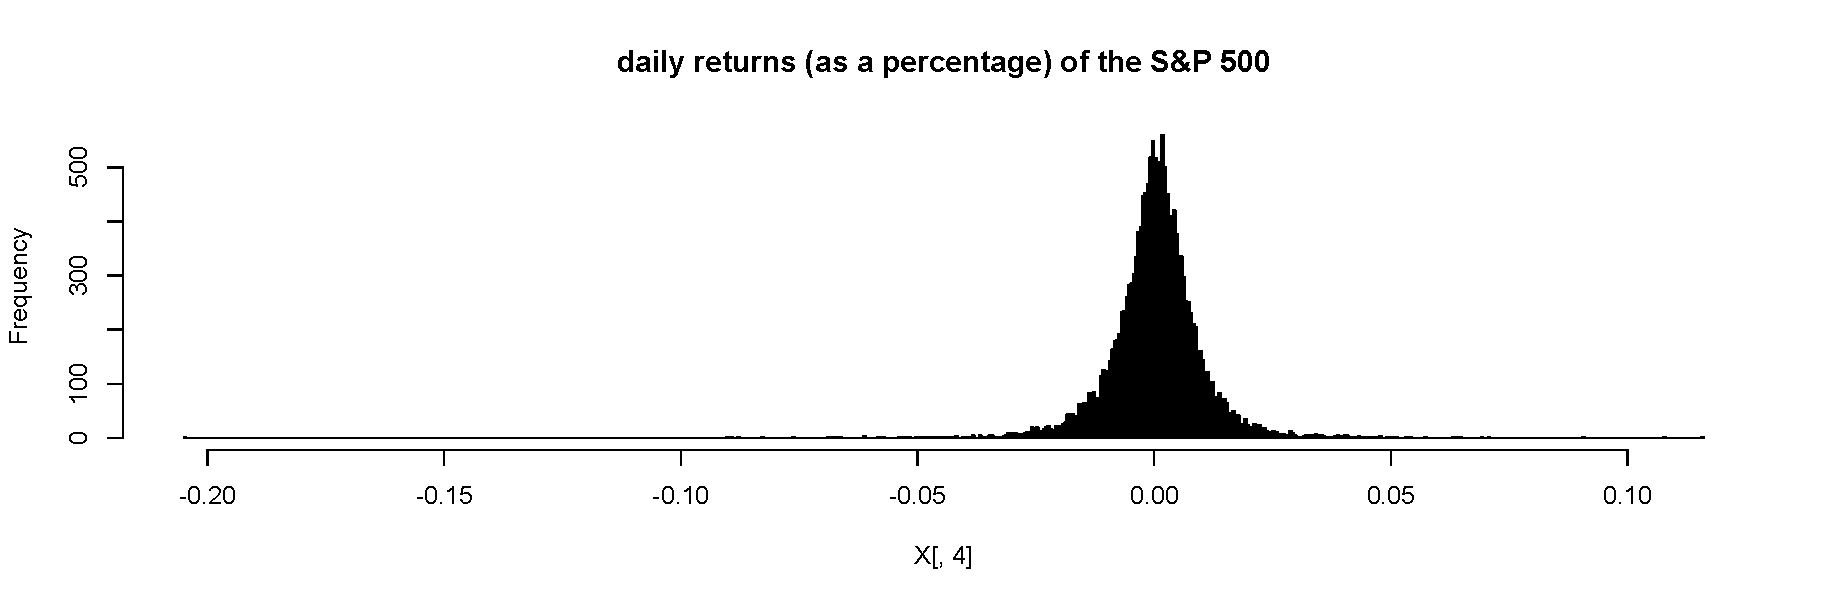
\includegraphics[width=7in]{daily_returns}
\end{figure}

%\begin{verbatim}
%X = read.csv('sp_tot_ret_price_1950.csv')
%n = nrow(X)
%n
%hist(X[,4], br = 1000, 
%  main = 'daily returns (as a percentage) of the S&P 500')
%\end{verbatim}

\intermediatesubproblem{Do you think the data is $\iid$? Explain.}\spc{1}
No because previous days can influence the days in the future. 

\intermediatesubproblem{Assume $\iid$ normal data regardless of what you wrote in (a) and (b). The sample average is $\xbar = 0.0003415$ and the sample standard deviation is $s = 0.0096$. Under an objective prior, give a 95\% credible region for the true mean daily return.}\spc{4}
\begin{align*}
    CR_{\theta,95\%} &= [\texttt{qnorm}(0.025, 0.0003415, \frac{0.0096^2}{16428}), 
        \texttt{qnorm}(0.975, 0.003415, \frac{0.0096^2}{16428})]\\
    & =[0.00341489, 0.00341511]
\end{align*}

\hardsubproblem{Give a 95\% credible region for \emph{tomorrow's} return using functions in Table~\ref{tab:eqs}.}\spc{4}
\begin{align*}
    CR_{95\%} &= [\texttt{qnorm}(0.025,  0.003415, \squared{0.0096}), \texttt{qnorm}(0.975, 0.003415,\squared{0.0096})]\\
    & =[0.0001608697, 0.0005221303]
\end{align*}

\end{enumerate}


\end{document}



\problem{This problem is about the normal-normal model using a \qu{semi-conjugate} prior. Assume $\Xoneton~|~\theta, \sigsq \iid \normnot{\theta}{\sigsq}$ throughout.}

\begin{enumerate}

\easysubproblem{If $\theta$ and $\sigsq$ are assumed to be independent, how can $\prob{\theta,~\sigsq}$ be factored?}\spc{1}

\easysubproblem{If $\prob{\theta} = \normnot{\mu_0}{\tausq}$ and $\prob{\sigsq} \sim \invgammanot{\overtwo{n_0}}{\overtwo{n_0 \sigsq_0}}$, find the kernel of the joint posterior, $\cprob{\theta,~\sigsq}{X}$}.\spc{4}

\hardsubproblem{Show that this kernel can be factored into the kernel of a normal where the leftover is \textit{not} the kernel of an inverse gamma. This is in the lecture notes.}\spc{12}

\hardsubproblem{[MA] Find the posterior mode of $\sigsq$ using $k(\sigsq~|~X)$.}\spc{5}

\hardsubproblem{Describe how you would sample from $k(\sigsq~|~X)$. Make all steps explicit and use the notation from Table~\ref{tab:eqs}.}\spc{10}

\hardsubproblem{Describe how you would sample from $\cprob{\theta,~\sigsq}{X}$. Make use of the sampling algorithm in the previous question. Make all steps explicit and use the notation from Table~\ref{tab:eqs}.}\spc{10}
 


\hardsubproblem{What are the two main disadvantages of grid sampling?}\spc{4}

\hardsubproblem{Why do you think the prior $\prob{\theta} = \normnot{\mu_0}{\tausq}$ and $\prob{\sigsq} \sim \invgammanot{\overtwo{n_0}}{\overtwo{n_0 \sigsq_0}}$ is called \qu{semi-conjugate}?}\spc{4}


\extracreditsubproblem{[MA] Find the MMSE of $\sigsq$}\spc{0}

\end{enumerate}



\end{document}


%%%%%%%%%%%%%%%%%%%%%%%%%%%%%%


\problem{These are questions about McGrayne's book, chapter 17 and the Epilogue.}

\begin{enumerate}

\easysubproblem{What do the computer scientists who adopted Bayesian methods care most about and whose view do they subscribe to? (p233)}\spc{1}

\easysubproblem{How was \qu{Stanley} able to cross the Nevada desert?}\spc{3}

\easysubproblem{What two factors are leading to the \qu{crumbling of the Tower of Babel?}}\spc{3}

\intermediatesubproblem{Does the brain work through iterative Bayesian modeling?}\spc{4}

\easysubproblem{According to Geman, what is the most powerful argument for Bayesian Statistics?}\spc{3}

\end{enumerate}







